\documentclass[sigconf,natbib=true,anonymous]{acmart}
%% WSDM 2027 — 9 pages + unlimited references + ethics
%% v3.1: expanded for page budget (protocol fig, multi-metric, shift, related, per-seed, RQ3, conclusion, appendix)

\settopmatter{printacmref=false}
\renewcommand\footnotetextcopyrightpermission[1]{}
\setcopyright{none}
\acmConference[WSDM'27]{Proceedings of the 20th ACM International Conference on Web Search and Data Mining}{February 15--19, 2027}{Hong Kong}
\acmYear{2027}
\acmDOI{}
\acmISBN{}

\usepackage{booktabs}
\usepackage{multirow}
\usepackage{amsmath,amssymb}
\usepackage{graphicx}
\usepackage{subcaption}
\usepackage{siunitx}
\usepackage{xspace}
\usepackage{enumitem}
\usepackage{microtype}
\usepackage{balance}
\usepackage{hyperref}

\newcommand{\tfidf}{\textsc{TF-IDF}\xspace}
\newcommand{\llm}{\textsc{LLM}\xspace}
\newcommand{\mv}{\textsc{MV}\xspace}
\newcommand{\base}{\textsc{SASRec}\xspace}

\begin{document}

\title{Do More Text Views Help?\\
A Leakage-Aware Evaluation of Text Representations\\
for Sequential Recommendation}

\author{Anonymous Author(s)}
\affiliation{%
  \institution{Anonymous Institution}
  \country{}}
\renewcommand{\shortauthors}{Anonymous}

%==============================================================================
\begin{abstract}
%==============================================================================
Text features are widely adopted to enhance sequential recommenders, yet conclusions about which representation is best almost universally come from leave-one-out (LOO) protocols that permit temporal leakage.
We conduct a controlled, leakage-aware study comparing four text representations---ID-only, cutoff-fit \tfidf, single-view \llm embeddings, and prompt-based multi-view \llm features---under global temporal split (GTS) with Last and Random target modes, as well as clean LOO, on three Amazon datasets (Beauty, Toys, Grocery).

Three findings emerge.
\textbf{(1)~Protocol changes conclusions.}
Under GTS-Last (warm targets), multi-view leads narrowly (Beauty MRR@10 $.0061$ vs.\ \tfidf $.0051$); under GTS-Random, \tfidf ranks first ($0.0139$ vs.\ MV $0.0134$); under LOO, \llm and multi-view appear strongest with 3--6$\times$ inflated absolutes.
The relative ordering of \tfidf, \llm, and multi-view is sensitive to target protocol---text consistently beats ID-only, but \emph{which} text is best depends on how evaluation targets are selected.
\textbf{(2)~No text variant is robustly dominant across temporal windows.}
Under GTS-Random, \tfidf is most stable across Main/Early windows; under GTS-Last, multi-view narrowly leads but all text variants fall within one standard deviation.
\textbf{(3)~Prompt multi-view gains are limited by inter-view redundancy.}
Pairwise CKA among four prompt views ranges 0.82--0.94, concatenated effective rank is 53--55\% of dimensionality, and leave-one-view-out changes MRR by at most 0.03 percentage points.
Meanwhile, CKA between \tfidf and any \llm view is only $\approx$0.19, indicating genuine lexical--semantic complementarity that multi-prompt stacking does not exploit.
\end{abstract}

\begin{CCSXML}
<ccs2012>
 <concept>
  <concept_id>10002951.10003317.10003347.10003350</concept_id>
  <concept_desc>Information systems~Recommender systems</concept_desc>
  <concept_significance>500</concept_significance>
 </concept>
 <concept>
  <concept_id>10002951.10003317.10003318.10003319</concept_id>
  <concept_desc>Information systems~Content ranking</concept_desc>
  <concept_significance>300</concept_significance>
 </concept>
</ccs2012>
\end{CCSXML}
\ccsdesc[500]{Information systems~Recommender systems}
\ccsdesc[300]{Information systems~Content ranking}

\keywords{Sequential Recommendation, Text Features, Temporal Evaluation, Multi-View Redundancy, Leakage-Aware Protocol}

\maketitle

%==============================================================================
\section{Introduction}
\label{sec:intro}
%==============================================================================

Sequential recommendation predicts a user's next item from historical interactions~\cite{kang2018sasrec,sun2019bert4rec,hidasi2016gru4rec}.
Item text---titles, descriptions, and LLM-generated semantics---is a standard way to enrich ID embeddings and enable cross-domain transfer~\cite{hou2022unisrec,bao2023tallrec}.
A natural working hypothesis is that \emph{richer text always helps}: LLM embeddings should beat bag-of-words, and multiple prompt-based views should beat a single view.

This hypothesis rests on fragile evaluation foundations.
Most text-enhanced sequential recommenders are validated with leave-one-out (LOO) splits that allow temporal overlap between training and test, inflating metrics and potentially distorting model comparisons~\cite{ji2023evaluation,sun2023reevaluation}.
Global temporal split (GTS) better simulates deployment but introduces additional design choices: the \emph{target-selection mode} (Last, Random, Successive, or All interactions per user in the test window) itself changes effective task difficulty and can alter model rankings~\cite{liang2024timetosplit}.
Prior work has studied split effects in general~\cite{meng2020temporal,ji2023evaluation}; we demonstrate that these effects are \emph{specifically decisive} for the \tfidf vs.\ \llm vs.\ multi-view comparison.

We conduct this study with strict leakage controls: all text features (\tfidf vocabulary/IDF, SVD, LLM center/whiten) are fit only on pre-cutoff items.
We compare five model variants on three Amazon datasets under GTS-Last (primary), GTS-Random (robustness check), and clean LOO (contrast), with an Early temporal window and UniSRec~\cite{hou2022unisrec} as external baseline.
We diagnose multi-view behavior with CKA~\cite{kornblith2019cka}, effective rank, and leave-one-view-out (LOOV).

\smallskip\noindent\textbf{Research questions.}
\begin{enumerate}[leftmargin=*,itemsep=1pt]
\item[\textbf{RQ1}] \emph{Protocol effect.}
Do clean LOO, GTS-Last, and GTS-Random change the absolute gains and relative ranking of \tfidf, single-view \llm, and prompt multi-view?
\item[\textbf{RQ2}] \emph{Temporal robustness.}
Can the conclusions drawn under the Main temporal window ($80\%$ cutoff) survive when the training window shrinks (Early, $60\%$ cutoff)?
\item[\textbf{RQ3}] \emph{Multi-view redundancy.}
Why do four prompt views not reliably outperform a single \llm view or even \tfidf, and where does genuine complementarity lie?
\end{enumerate}

\smallskip\noindent\textbf{Contributions.}
\begin{enumerate}[leftmargin=*,itemsep=1pt]
\item A leakage-aware comparison on three datasets showing that the same checkpoints yield different text-representation rankings under different target modes (Last vs.\ Random vs.\ LOO): text always beats ID, but \emph{which} text is best is protocol-sensitive.
\item Cross-window evidence that no single text variant robustly dominates across Main and Early temporal windows---\tfidf is most stable under GTS-Random, multi-view marginally leads under GTS-Last, but differences are within noise.
\item A triangulated redundancy analysis (CKA + effective rank + LOOV) jointly explaining limited multi-view gains, while identifying lexical--semantic complementarity (TF vs.\ LLM, CKA$\approx$0.19) as an unexploited axis.
\end{enumerate}

%==============================================================================
\section{Related Work}
\label{sec:related}
%==============================================================================

\paragraph{Text-enhanced sequential recommendation.}
Early systems fused bag-of-words or review text with collaborative filtering~\cite{wang2015cdl,salton1988termweighting}.
Modern approaches encode titles and descriptions with pretrained language models for cross-domain transfer~\cite{hou2022unisrec,hou2023vqrec,geng2022p5,bao2023tallrec}.
UniSRec learns transferable item representations from text and adapts them via a lightweight MoE~\cite{hou2022unisrec}; VQ-Rec quantizes textual embeddings for transfer~\cite{hou2023vqrec}; P5 casts recommendation as language modeling~\cite{geng2022p5}; TALLRec aligns LLMs to ranking via instruction tuning~\cite{bao2023tallrec}.
These systems typically report LOO or loosely specified temporal protocols.
We do \emph{not} propose a new architecture; we ask whether stronger text encoders and more views remain advantageous once temporal leakage is controlled under a fixed backbone.

\paragraph{LLM-based item representations.}
Beyond architecture papers, a growing practice is to treat LLM embeddings as drop-in item features---either as a single view (title/description) or as multiple prompt-conditioned views that supposedly capture complementary facets (function, audience, style).
Our study isolates this representation choice from architectural novelty: the same SASRec backbone and fusion pipeline are held fixed while only the text source changes (\tfidf, single-view \llm, or four-view \llm).

\paragraph{Evaluation protocols and temporal leakage.}
Sampled metrics distort rankings~\cite{krichene2020sampledmetrics}; LOO vs.\ time-based splits change absolute scores and can alter model selection~\cite{ji2023evaluation,sun2023reevaluation,meng2020temporal}.
Within GTS, target-selection mode matters: \citet{liang2024timetosplit} show that Successive best approximates online next-item prediction but is expensive; Last is a deterministic low-cost proxy; Random has highest rank-correlation with Successive when sampling seeds are fixed; and All packs multiple items into one ground-truth set, introducing task mismatch and the weakest correlation with Successive.
We specialize this finding to text representations: protocol changes conclusions \emph{precisely because} \tfidf, \llm, and \mv respond differently to distribution shift.
Matching validation and test target modes (both Last, or both Random) is also recommended for reliable model selection~\cite{liang2024timetosplit}; our Early-window experiments keep this alignment.

\paragraph{Multi-view learning and representation redundancy.}
Multi-view theory holds that views must be \emph{useful and complementary}; more views do not guarantee benefit~\cite{xu2013multiview}.
CKA~\cite{kornblith2019cka} measures representational similarity of Gram structures and can detect redundancy even when instance-level pairwise cosine is moderate.
Effective rank (entropy of normalized singular values) quantifies how much of a representation's nominal dimensionality is actually used.
We combine CKA, effective rank, and LOOV---not CKA alone---to explain limited multi-view gains.

\paragraph{Information geometry of embeddings.}
Singular-value concentration and anisotropy are known failure modes of pretrained text embeddings~\cite{ethayarajh2019contextual}.
Our effective-rank analysis connects this literature to sequential recommendation: concatenating four prompt views that share the same encoder yields ER/dim $\approx$0.53, whereas a lexical \tfidf SVD of the same dimension retains ER/dim $\approx$0.98.

%==============================================================================
\section{Controlled Study Setup}
\label{sec:setup}
%==============================================================================

\subsection{Temporal Protocols}
\label{sec:protocol}

\paragraph{GTS-Last (primary).}
Interactions are globally ordered by timestamp; RecBole's \texttt{TS} split~\cite{zhao2021recbole} with $[0.8,0.1,0.1]$ (Main) or $[0.6,0.1,0.3]$ (Early).
After sequential augmentation, each user contributes only their \textbf{chronologically last} test interaction to evaluation (one target per user), following the ``predict the user's last item'' paradigm recommended by \citet{liang2024timetosplit}.

\paragraph{GTS-Random (robustness check).}
Same checkpoints; each user contributes one \textbf{uniformly random} test interaction (target-sampling seed fixed at 42 for reproducibility).
Random has the highest rank-correlation with Successive~\cite{liang2024timetosplit} and serves as a cross-check.

\paragraph{Clean LOO (contrast).}
Leave-one-out (last-3 interactions per user as train/valid/test; no time cutoff).
Included only to quantify the protocol gap; \emph{not} used for primary conclusions.

\paragraph{GTS-All (appendix).}
All post-cutoff targets per user; relegated to Appendix~\ref{app:gts-all} due to task-mismatch concerns~\cite{liang2024timetosplit}.

\paragraph{Leakage controls.}
\tfidf vocabulary/IDF, SVD projection, and LLM center/whitening are fit only on items appearing before the training cutoff.
Evaluation filters users with $\ge 5$ training interactions.
Main tables report \textbf{warm-target} results (target $\in$ train catalog); all-target and unseen diagnostics appear in Appendix~\ref{app:alltarget}.

\subsection{Text Representations and Models}
\label{sec:models}

All variants share a \base~\cite{kang2018sasrec} backbone ($d{=}64$, 2 layers, 2 attention heads).

\begin{itemize}[leftmargin=*,itemsep=1pt]
\item \textbf{ID}: ID embeddings only.
\item \textbf{TF}: train-cutoff \tfidf $\to$ SVD 256-d $\to$ lightweight projection head + InfoNCE alignment~\cite{oord2018cpc}.
\item \textbf{LLM}: single-view Qwen2.5-7B~\cite{qwen2024qwen25} item embedding (train-cutoff centered and whitened), same fusion pipeline.
\item \textbf{MV}: four prompt views (Description / Function / Audience / Style) $\to$ per-view 64-d projections $\to$ 256-d concatenation $\to$ shared projection; no cross-attention.
\item \textbf{UniSRec}~\cite{hou2022unisrec}: external text-enhanced sequential baseline with the same TS-whitened LLM embeddings and identical eval filter.
\end{itemize}

TF/LLM/MV use two-phase training: Phase~A (text-head warmup via InfoNCE), then Phase~B (joint BPR~\cite{rendle2009bpr} + InfoNCE fine-tuning).
Hyperparameters for the Early window are frozen from Main (no re-tuning).

\subsection{Datasets}

Amazon Beauty, Toys \& Games, and Grocery \& Gourmet Food~\cite{mcauley2015amazon,ni2019amazon}:
\begin{itemize}[leftmargin=*,itemsep=1pt]
\item \textbf{Beauty}: 1.21M users, 259K items, 2.02M interactions.
\item \textbf{Toys}: 1.28M users, 336K items, 2.25M interactions.
\item \textbf{Grocery}: 768K users, 172K items, 1.30M interactions (same-platform replication; not claimed as domain diversity).
\end{itemize}

\subsection{Evaluation Details}

Full-ranking Hit@10, NDCG@10, MRR@10~\cite{krichene2020sampledmetrics}.
Main tables: MRR@10, mean$\pm$sample-std over 3 seeds (42, 2024, 2026); NDCG/Hit reported as secondary metrics.
All runs on a single NVIDIA RTX 5090; per-model training: 15--65~min.

%==============================================================================
\section{RQ1: Protocol Changes Rankings}
\label{sec:rq1}
%==============================================================================

\begin{table}[t]
\centering
\caption{%
Protocol contrast --- warm-target MRR@10 (3-seed mean$\pm$std, min5 filter).
\textbf{Bold}: best \emph{text} method per row.
The winner changes with the protocol: GTS-Last favors MV; GTS-Random favors TF; LOO favors LLM$\approx$MV.
Text always beats ID regardless of protocol.%
}
\label{tab:protocol}
\small
\setlength{\tabcolsep}{2.8pt}
\begin{tabular}{@{}llccccc@{}}
\toprule
Dataset & Protocol & ID & TF & LLM & MV & UniSRec \\
\midrule
\multirow{3}{*}{Beauty}
 & GTS-Last  & .0032\tiny{$\pm$.0006} & .0051\tiny{$\pm$.0008} & .0059\tiny{$\pm$.0005} & \textbf{.0061}\tiny{$\pm$.0005} & .0052\tiny{$\pm$.0002} \\
 & GTS-Rand  & .0081\tiny{$\pm$.0003} & \textbf{.0139}\tiny{$\pm$.0013} & .0130\tiny{$\pm$.0015} & .0134\tiny{$\pm$.0011} & .0098\tiny{$\pm$.0001} \\
 & LOO       & .0175\tiny{$\pm$.0004} & .0251\tiny{$\pm$.0002} & \textbf{.0254}\tiny{$\pm$.0004} & .0253\tiny{$\pm$.0004} & --- \\
\midrule
\multirow{3}{*}{Toys}
 & GTS-Last  & .0031\tiny{$\pm$.0002} & .0040\tiny{$\pm$.0005} & .0035\tiny{$\pm$.0002} & \textbf{.0042}\tiny{$\pm$.0006} & .0041\tiny{$\pm$.0001} \\
 & GTS-Rand  & .0096\tiny{$\pm$.0006} & \textbf{.0146}\tiny{$\pm$.0006} & .0140\tiny{$\pm$.0007} & .0141\tiny{$\pm$.0008} & .0103\tiny{$\pm$.0006} \\
 & LOO       & .0152\tiny{$\pm$.0005} & .0247\tiny{$\pm$.0006} & .0258\tiny{$\pm$.0012} & \textbf{.0258}\tiny{$\pm$.0028} & --- \\
\midrule
\multirow{2}{*}{Grocery}
 & GTS-Last  & .0030\tiny{$\pm$.0012} & .0046\tiny{$\pm$.0006} & .0047\tiny{$\pm$.0005} & \textbf{.0058}\tiny{$\pm$.0007} & --- \\
 & GTS-Rand  & .0044\tiny{$\pm$.0012} & \textbf{.0085}\tiny{$\pm$.0014} & .0079\tiny{$\pm$.0006} & \textbf{.0085}\tiny{$\pm$.0007} & --- \\
\bottomrule
\end{tabular}
\end{table}

\begin{figure}[t]
\centering
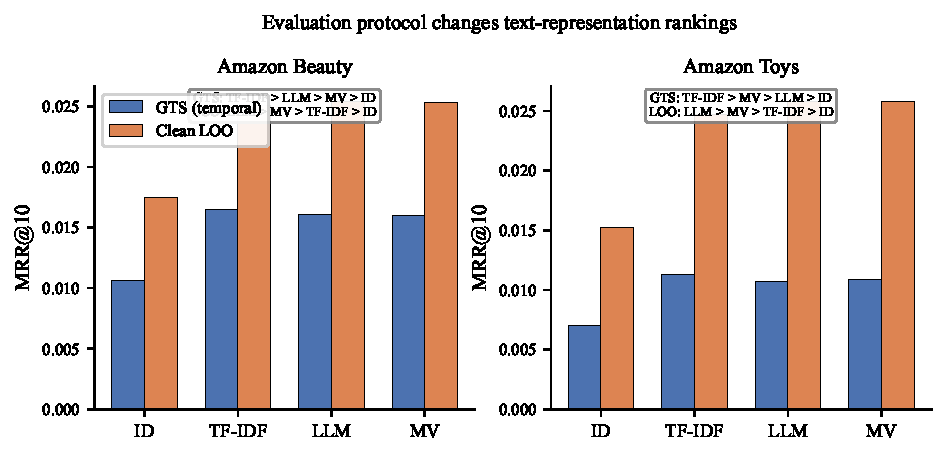
\includegraphics[width=\linewidth]{figures/fig_protocol_contrast.pdf}
\caption{%
Protocol contrast on Beauty and Toys (3-seed mean MRR@10).
Clean LOO inflates absolutes and favors LLM/MV; temporal GTS lowers scores and can change the ranking among text methods.
Table~\ref{tab:protocol} further shows that within GTS, Last vs.\ Random also flips the winner.%
}
\label{fig:protocol}
\end{figure}

\begin{table}[t]
\centering
\caption{%
GTS-Last warm NDCG@10 and Hit@10 (3-seed mean$\pm$std).
Ranking is broadly consistent with MRR, with UniSRec competitive on Hit.%
}
\label{tab:ndcg_hit}
\small
\setlength{\tabcolsep}{3pt}
\begin{tabular}{@{}llccccc@{}}
\toprule
Dataset & Metric & ID & TF & LLM & MV & UniSRec \\
\midrule
\multirow{2}{*}{Beauty}
 & NDCG & .0047\tiny{$\pm$.0007} & .0072\tiny{$\pm$.0011} & \textbf{.0084}\tiny{$\pm$.0006} & .0083\tiny{$\pm$.0005} & .0081\tiny{$\pm$.0003} \\
 & Hit  & .0098\tiny{$\pm$.0013} & .0140\tiny{$\pm$.0019} & .0167\tiny{$\pm$.0013} & .0157\tiny{$\pm$.0010} & \textbf{.0180}\tiny{$\pm$.0007} \\
\midrule
\multirow{2}{*}{Toys}
 & NDCG & .0046\tiny{$\pm$.0004} & .0056\tiny{$\pm$.0006} & .0046\tiny{$\pm$.0002} & .0057\tiny{$\pm$.0011} & \textbf{.0067}\tiny{$\pm$.0005} \\
 & Hit  & .0098\tiny{$\pm$.0013} & .0108\tiny{$\pm$.0011} & .0084\tiny{$\pm$.0004} & .0108\tiny{$\pm$.0027} & \textbf{.0154}\tiny{$\pm$.0023} \\
\midrule
\multirow{2}{*}{Grocery}
 & NDCG & .0048\tiny{$\pm$.0019} & .0062\tiny{$\pm$.0004} & .0063\tiny{$\pm$.0005} & \textbf{.0077}\tiny{$\pm$.0007} & --- \\
 & Hit  & .0107\tiny{$\pm$.0041} & .0117\tiny{$\pm$.0009} & .0117\tiny{$\pm$.0007} & \textbf{.0136}\tiny{$\pm$.0007} & --- \\
\bottomrule
\end{tabular}
\end{table}

\begin{table}[t]
\centering
\caption{%
Per-seed GTS-Last warm MRR@10 (seeds 42 / 2024 / 2026).
Variance is visible; MV's lead is small and seed-dependent.%
}
\label{tab:perseed}
\small
\setlength{\tabcolsep}{3.5pt}
\begin{tabular}{@{}llccccc@{}}
\toprule
Dataset & Seed & ID & TF & LLM & MV & UniSRec \\
\midrule
\multirow{3}{*}{Beauty}
 & 42    & .0038 & .0042 & .0054 & .0058 & .0050 \\
 & 2024  & .0032 & .0053 & .0060 & .0058 & .0054 \\
 & 2026  & .0026 & .0059 & .0064 & .0067 & .0051 \\
\midrule
\multirow{3}{*}{Toys}
 & 42    & .0033 & .0045 & .0037 & .0035 & .0042 \\
 & 2024  & .0030 & .0038 & .0032 & .0042 & .0042 \\
 & 2026  & .0029 & .0036 & .0036 & .0048 & .0041 \\
\bottomrule
\end{tabular}
\end{table}

Table~\ref{tab:protocol} and Figure~\ref{fig:protocol} present the central finding.
The key insight is \emph{not} that one text representation always wins, but that their \textbf{relative ordering is sensitive to the target-selection protocol}:

\begin{itemize}[leftmargin=*,itemsep=1pt]
\item \textbf{GTS-Last}: MV leads on all three datasets (Beauty $.0061$, Toys $.0042$, Grocery $.0058$), but the margin over LLM is small and often within one std (Table~\ref{tab:perseed}).
\item \textbf{GTS-Random}: TF leads on Beauty/Toys ($.0139$ / $.0146$) and ties MV on Grocery ($.0085$).
\item \textbf{LOO}: absolute MRR inflates 3--6$\times$ vs.\ GTS-Last; ranking becomes LLM $\approx$ MV $\ge$ TF.
\end{itemize}

Table~\ref{tab:ndcg_hit} shows that NDCG@10 largely agrees with MRR rankings under GTS-Last, while Hit@10 elevates UniSRec on Beauty/Toys---another reminder that metric choice interacts with protocol.
We therefore treat MRR as the primary ranking metric and report NDCG/Hit for completeness.

\paragraph{Implications.}
The \emph{same checkpoints} (same trained weights) produce different winners when evaluated with Last vs.\ Random target selection---a pure protocol artifact.
This demonstrates that claims of text-representation superiority are unreliable without specifying the target mode.
All text methods consistently and substantially outperform ID-only ($+$50--100\% relative) regardless of protocol, confirming the value of text features in general.
The most accurate summary of our data is therefore: \emph{text vs.\ ID is robust; TF vs.\ LLM vs.\ MV is protocol-sensitive}.

\paragraph{UniSRec as external baseline.}
Under identical GTS-Last + min5 + warm filter, UniSRec scores $0.0052$ (Beauty) and $0.0041$ (Toys)---between ID and TF on MRR, but stronger on Hit (Table~\ref{tab:ndcg_hit}).
Previously reported ``UniSRec wins'' arose from inconsistent evaluation filters (Appendix~\ref{app:unisrec}).

%==============================================================================
\section{RQ2: Temporal Robustness}
\label{sec:rq2}
%==============================================================================

\begin{table}[t]
\centering
\caption{%
Main ($80\%$ cutoff) vs.\ Early ($60\%$ cutoff) on Beauty --- warm MRR@10 (3-seed mean$\pm$std).
Hyperparameters frozen from Main.
Under GTS-Random, TF is most stable; under GTS-Last, MV leads but within overlapping CIs.%
}
\label{tab:early}
\small
\begin{tabular}{@{}lccc@{}}
\toprule
Window / eval mode & TF & LLM & MV \\
\midrule
Main, GTS-Last    & .0051\tiny{$\pm$.0008} & .0059\tiny{$\pm$.0005} & \textbf{.0061}\tiny{$\pm$.0005} \\
Early60, GTS-Last & .0026\tiny{$\pm$.0004} & .0023\tiny{$\pm$.0002} & \textbf{.0032}\tiny{$\pm$.0005} \\
\midrule
Main, GTS-Rand    & \textbf{.0139}\tiny{$\pm$.0013} & .0130\tiny{$\pm$.0015} & .0134\tiny{$\pm$.0011} \\
Early60, GTS-Rand & \textbf{.0061}\tiny{$\pm$.0004} & .0061\tiny{$\pm$.0003} & .0056\tiny{$\pm$.0002} \\
\bottomrule
\end{tabular}
\end{table}

\begin{table}[t]
\centering
\caption{%
Temporal distribution shift (valid$\to$test, Main GTS).
Reported as \emph{associations} with the observed Main$\to$Early performance drop (50--60\%), not causal claims.%
}
\label{tab:shift}
\small
\setlength{\tabcolsep}{4pt}
\begin{tabular}{@{}lccc@{}}
\toprule
Dataset & Unseen targets & Pop mean (V$\to$T) & Pop median (V$\to$T) \\
\midrule
Beauty  & 31.9\% & $112.8 \to 101.8$ & $21 \to 15$ \\
Toys    & 40.8\% & $144.7 \to 119.1$ & $18 \to 11$ \\
Grocery & 29.6\% & $87.3 \to 76.9$ & $16 \to 12$ \\
\bottomrule
\end{tabular}
\end{table}

\begin{table}[t]
\centering
\caption{%
Target popularity-bucket composition (valid$\to$test, Main GTS).
Head share drops while unseen share rises---concurrent with absolute metric degradation.%
}
\label{tab:bucket}
\small
\setlength{\tabcolsep}{3.5pt}
\begin{tabular}{@{}llcccc@{}}
\toprule
Dataset & Split & Head & Mid & Low & Unseen \\
\midrule
\multirow{2}{*}{Beauty}
 & Valid & 63.1\% & 15.9\% & 9.7\% & 11.3\% \\
 & Test  & 56.6\% & 14.9\% & 10.7\% & 17.8\% \\
\midrule
\multirow{2}{*}{Toys}
 & Valid & 60.1\% & 16.3\% & 10.6\% & 13.0\% \\
 & Test  & 52.3\% & 15.5\% & 11.0\% & 21.3\% \\
\bottomrule
\end{tabular}
\end{table}

Table~\ref{tab:early} shows that shrinking the training window to 60\% preserves the general pattern but amplifies uncertainty: absolute scores drop 50--60\% across all models.
Table~\ref{tab:shift} documents concurrent shifts: 30--41\% of test targets are items absent from training, and target popularity declines.
Table~\ref{tab:bucket} further decomposes the shift into popularity buckets: from valid to test, head share falls by $\approx$6--8 points while unseen share rises by $\approx$6--8 points on both Beauty and Toys.
Catalog novelty ratios tell the same story (Beauty test new-item ratio 27.3\%; Toys 32.8\%).

Eligible users with history length $\ge 5$ remain substantial (Beauty: 39.5K; Toys: 44.0K), and median history length is stable (8 on both valid and test), so the degradation is not explained by shorter sequences alone.
Instead, the composition of \emph{targets} changes: more cold/unseen items and fewer head items.

The most stable conclusion across both windows is:
(i)~under GTS-Random, \tfidf leads or ties in both Main and Early;
(ii)~under GTS-Last, MV narrowly leads in both, but differences are within one std.
\textbf{No single text variant robustly dominates} once both protocol choice and temporal window are varied.
This sensitivity is the core phenomenon, not the dominance of any one method.
We emphasize association rather than causation: the shift statistics co-occur with the Main$\to$Early drop, but we do not claim that unseen share alone \emph{causes} the ranking pattern.

%==============================================================================
\section{RQ3: Why Limited Multi-View Gain}
\label{sec:rq3}
%==============================================================================

\begin{figure}[t]
\centering
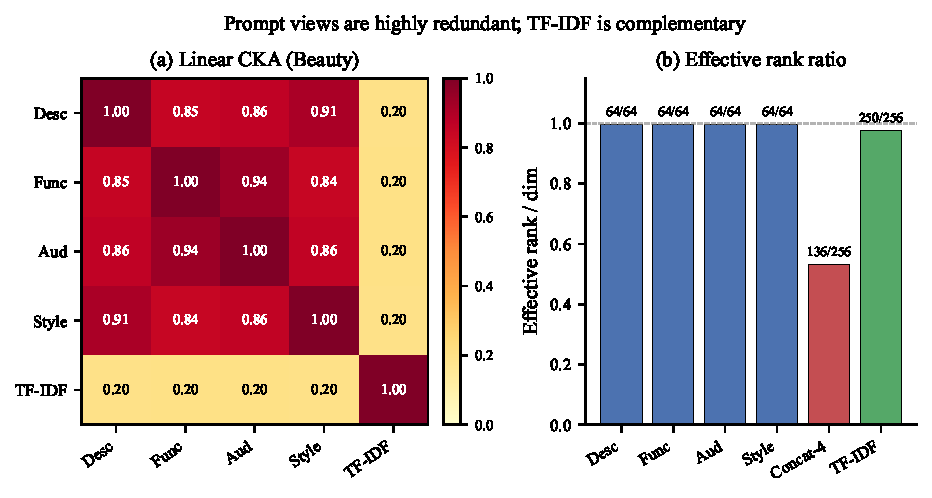
\includegraphics[width=\linewidth]{figures/fig_cka_heatmap.pdf}
\caption{%
Representation analysis on Beauty (3 random item subsamples of 3{,}000 each, mean$\pm$std).
\textbf{(a)}~Pairwise CKA: LLM views show high mutual similarity (0.84--0.94); TF--LLM CKA is low ($\approx$0.20).
\textbf{(b)}~Effective rank: 4-view concat 136/256 (53\%) vs.\ TF-IDF 250/256 (98\%).%
}
\label{fig:cka}
\end{figure}

\begin{table}[t]
\centering
\caption{%
Inter-view CKA (3 subsamples of 3K items, mean$\pm$std).
All LLM view pairs exceed 0.82; TF-IDF vs.\ any LLM view stays below 0.20.%
}
\label{tab:cka}
\small
\setlength{\tabcolsep}{4pt}
\begin{tabular}{@{}lcc@{}}
\toprule
View Pair & Beauty & Toys \\
\midrule
Description--Function  & $.846 \pm .001$ & $.834 \pm .001$ \\
Description--Audience  & $.860 \pm .001$ & $.856 \pm .002$ \\
Description--Style     & $.914 \pm .000$ & $.904 \pm .001$ \\
Function--Audience     & $.940 \pm .000$ & $.921 \pm .001$ \\
Function--Style        & $.843 \pm .001$ & $.818 \pm .002$ \\
Audience--Style        & $.859 \pm .001$ & $.838 \pm .002$ \\
\midrule
\emph{TF-IDF vs.\ LLM view (range)} & $.196$--$.201$ & $.184$--$.189$ \\
\bottomrule
\end{tabular}
\end{table}

\begin{table}[t]
\centering
\caption{%
Effective rank (Beauty/Toys, 3 subsamples).
4-view concat occupies only 53--55\% of its nominal dimensionality.%
}
\label{tab:effrank}
\small
\begin{tabular}{@{}lccc@{}}
\toprule
Representation & Dim & ER (Beauty) & ER (Toys) \\
\midrule
Single LLM view (avg) & 64 & 63.7 (99.5\%) & 63.6 (99.4\%) \\
4-view concat & 256 & 136.1 (\textbf{53.2\%}) & 141.2 (\textbf{55.2\%}) \\
TF-IDF (SVD) & 256 & 249.9 (97.6\%) & 251.4 (98.2\%) \\
\bottomrule
\end{tabular}
\end{table}

\begin{table}[t]
\centering
\caption{%
Leave-one-view-out (zero-mask, seed~42, GTS-All, min5 filter).
$\Delta$: MRR@10 change vs.\ full 4-view model.
Maximum $|\Delta|$ is 0.00034 ($<$2.2\% relative).%
}
\label{tab:loov}
\small
\setlength{\tabcolsep}{3.5pt}
\begin{tabular}{@{}lccccc@{}}
\toprule
Dataset & Full MRR & $-$Desc & $-$Func & $-$Aud & $-$Style \\
\midrule
Beauty & .01591 & $-$.00006 & $+$.00011 & $-$.00016 & $-$.00034 \\
Toys   & .01018 & $-$.00019 & $-$.00011 & $-$.00012 & $-$.00015 \\
\bottomrule
\end{tabular}
\end{table}

We address RQ3 by triangulating three complementary analyses.
No single measure suffices: CKA captures structural similarity but cannot alone prove task-irrelevance~\cite{kornblith2019cka}; effective rank measures dimensionality utilization; LOOV measures downstream impact.
Together they provide converging evidence that prompt multi-view gains are limited by inter-view redundancy.

\paragraph{(1) High inter-view CKA.}
Table~\ref{tab:cka} and Figure~\ref{fig:cka}(a) show that all six LLM view pairs have CKA $\ge 0.82$ (Beauty 0.84--0.94; Toys 0.82--0.92).
The four prompt views, generated from the same encoder applied to the same item text with different instructions, encode highly similar relational structures.
In contrast, TF-IDF vs.\ any LLM view yields CKA $\approx$0.19--0.20 (Beauty) and 0.18--0.19 (Toys)---a qualitatively different regime indicating genuinely complementary information.

\paragraph{(2) Pairwise cosine vs.\ CKA.}
Mean pairwise cosine between prompt views is often moderate or near zero (e.g., Description--Function $\approx -0.01$ on Beauty), while Function--Audience reaches $\approx 0.42$.
This does \emph{not} contradict high CKA: cosine measures instance-level alignment of vectors, whereas CKA compares Gram-matrix geometry across the item set~\cite{kornblith2019cka}.
Views can have low average cosine yet still induce nearly isomorphic similarity structures---precisely the failure mode of ``semantic paraphrasing'' via prompts.
We therefore treat CKA as the primary similarity diagnostic and use cosine only as a complementary check, never as standalone proof of redundancy.

\paragraph{(3) Low effective rank of concatenated views.}
Table~\ref{tab:effrank} and Figure~\ref{fig:cka}(b) show that concatenating four 64-d views into 256 dimensions yields effective rank of only 136 (Beauty) and 141 (Toys), occupying 53--55\% of the available capacity.
Nearly half the dimensions are ``consumed'' by redundant structure.
TF-IDF at the same 256-d has effective rank $\ge$250 (97--98\%), utilizing almost all capacity.
An automated diagnosis on the same representations flags \texttt{REDUNDANT} / \texttt{collapse=True}, consistent with the quantitative thresholds above.

\paragraph{(4) Negligible LOOV impact.}
Table~\ref{tab:loov} shows that zeroing any single view has minimal downstream effect: maximum $|\Delta|$ = 0.00034 (Style on Beauty, 2.1\% relative to full MV).
On Toys, all drops yield $|\Delta| \le 0.00019$.
Given the other three views, any one view's marginal information is near-zero.

\paragraph{Where does redundancy originate?}
Our CKA and effective-rank numbers are computed on \emph{post-projection} 64-d view embeddings (after SVD/whitening toward the model input).
A remaining open question is whether the high inter-view CKA already exists in the raw 4096-d Qwen embeddings, or whether projection collapses otherwise complementary signals.
If high CKA appears pre-projection, redundancy is attributable to prompt semantic paraphrasing; if it appears only post-projection, preprocessing is implicated.
We leave this offline audit to future work (Section~\ref{sec:future}); expanding view dimensionality to $4\times256$ is \emph{not} justified by current evidence, which points to redundancy rather than capacity shortage (Table~\ref{tab:cost}).

\paragraph{Synthesis.}
The analyses converge: prompt views encode overlapping semantics, leading to dimensionality collapse and negligible per-view contribution.
This is consistent with multi-view theory---views derived from a single source via semantic paraphrasing fail the complementarity condition~\cite{xu2013multiview}.
The genuine complementarity in our system lies between lexical \tfidf and semantic \llm (CKA$\approx$0.19), but it is not harvested by naive multi-prompt stacking---the MV model simply replicates similar semantic structures four times instead of combining lexical and semantic axes.

%==============================================================================
\section{Discussion and Limitations}
\label{sec:discussion}
%==============================================================================

\paragraph{Practitioner implications.}
\begin{enumerate}[leftmargin=*,itemsep=2pt]
\item Report text-representation comparisons under GTS with explicit target mode.  LOO can reverse rankings and inflate metrics 3--6$\times$.
\item Start with cutoff-fit \tfidf as a strong baseline.  Under GTS-Random it is consistently first; under GTS-Last it is competitive but may trail LLM/MV.
\item A single \llm view typically matches four prompt views; diagnose redundancy before scaling views.
\item Genuine complementarity (TF vs.\ LLM, CKA$\approx$0.19) suggests hybrid TF+LLM fusion as a more promising direction than expanding prompt views.
\item Do not overclaim a single ``best'' text representation across protocols; report Last and Random (or Successive) side by side.
\end{enumerate}

\paragraph{Limitations.}
\begin{itemize}[leftmargin=*,itemsep=1pt]
\item \textbf{Warm-target scope.}
Our models lack content-only zero-shot fallback; warm-target evaluation is thus the fairest comparison, but it excludes 30--41\% of real test items.
\item \textbf{Static metadata.}
We use fixed product titles/descriptions; temporally evolving text (e.g., reviews, trending tags) could change the TF/LLM balance.
\item \textbf{Amazon-only domain.}
All three datasets are Amazon subcategories.  Grocery is a same-platform replication, not a solution to domain diversity.
\item \textbf{GTS-Random reproducibility.}
We use a single fixed target-sampling seed (42).  Averaging over multiple sampling seeds would tighten estimates~\cite{liang2024timetosplit}.
\item \textbf{Redundancy locus.}
CKA uses post-projection 64-d embeddings; a raw 4096-d audit remains future work.
\item \textbf{Successive not fully run.}
We rely on Last/Random as proxies; a sampled-user Successive sanity check would further validate protocol choice.
\end{itemize}

\paragraph{Cost analysis.}
\begin{table}[t]
\centering
\caption{Parameter count and inference cost (seed~42).  MV adds $<$1\% parameters.}
\label{tab:cost}
\small
\begin{tabular}{@{}lcc@{}}
\toprule
Model & Params (M) & ms/sample \\
\midrule
ID / TF / LLM / MV & 67.2 / 67.4 / 67.6 / 67.7 & 0.02 \\
UniSRec & 67.7 & 0.04 \\
\bottomrule
\multicolumn{3}{@{}l}{\footnotesize Beauty; Toys is $\sim$87M due to larger vocab (ranking identical).}
\end{tabular}
\end{table}

Table~\ref{tab:cost} confirms multi-view failure is not a capacity issue.  All variants have effectively the same parameter budget and inference cost.

%==============================================================================
\section{Conclusion}
\label{sec:conclusion}
%==============================================================================

We conducted a leakage-aware controlled study of text representations for sequential recommendation, structured as an empirical investigation rather than a model-proposal paper.
Three conclusions emerge for the community:

\begin{enumerate}[leftmargin=*,itemsep=1pt]
\item \textbf{Protocol matters.}
The relative ordering of \tfidf, single-view \llm, and prompt multi-view depends on the GTS target mode.
Text features consistently outperform ID-only, but which text is best requires specifying the evaluation protocol.
\item \textbf{No text variant is robustly dominant.}
Across temporal windows, the sensitivity persists---\tfidf is most stable under Random, MV narrowly leads under Last, but all are within noise margins.
\item \textbf{Multi-view gains are limited by inter-view redundancy.}
CKA, effective rank, and LOOV jointly show that prompt views encode overlapping semantics; genuine complementarity lies between lexical and semantic features.
\end{enumerate}

These findings matter because text-enhanced sequential recommendation is increasingly treated as an LLM upgrade problem.
Our evidence suggests the community should first lock the temporal protocol, then diagnose representation redundancy, before investing in additional prompt views or fusion modules.
The practical default under leakage-aware evaluation is: report GTS-Last (and Random as a check), keep cutoff-fit \tfidf as a mandatory baseline, and treat multi-view LLM features as a hypothesis to be tested---not a free upgrade.

\section{Future Work}
\label{sec:future}

Several directions follow naturally from the limitations above.
\begin{enumerate}[leftmargin=*,itemsep=1pt]
\item \textbf{Hybrid TF+LLM fusion} that targets the lexical--semantic complementarity axis (CKA$\approx$0.19) rather than expanding prompt views.
\item \textbf{Pre- vs.\ post-projection redundancy audit} on raw 4096-d Qwen embeddings vs.\ 64-d projected views, to locate whether redundancy is prompt-induced or compression-induced.
\item \textbf{GTS-Successive evaluation} at sampled-user scale, to validate Last/Random as proxies for online next-item prediction~\cite{liang2024timetosplit}.
\item \textbf{Multi-seed GTS-Random} averaging over fixed target-sampling seeds for tighter ranking estimates.
\item \textbf{Non-Amazon domains} with reliable timestamps, to test whether protocol sensitivity generalizes beyond product catalogs.
\end{enumerate}

\section*{Ethical Considerations}
This work uses public Amazon review datasets with no personally identifiable attributes beyond standard user/item IDs.
Potential concerns include reinforcing popularity bias under temporal shift and inheriting biases from LLM-generated text features.
We mitigate the former by reporting warm-target stratified diagnostics and the latter by treating multi-view LLM features as an empirical object of study rather than a recommended default.
No human subjects were involved.

\begin{acks}
Anonymous for review.
\end{acks}

\bibliographystyle{ACM-Reference-Format}
\bibliography{refs}

%==============================================================================
\appendix
%==============================================================================

\section{GTS-All Results}
\label{app:gts-all}

Main tables use GTS-Last (one last target per user).
GTS-All evaluates all post-cutoff targets (Beauty: 4{,}520 users $\to$ 12{,}001 samples, avg 2.65/user; Toys: 4{,}873 users $\to$ 13{,}186, avg 2.71/user).

\begin{table}[h]
\centering
\caption{GTS-All warm MRR@10 (3-seed mean).  TF dominates under All.}
\label{tab:gts-all}
\small
\begin{tabular}{@{}lccccc@{}}
\toprule
Dataset & ID & TF & LLM & MV & UniSRec \\
\midrule
Beauty & .0156 & \textbf{.0242} & .0236 & .0236 & .0123 \\
Toys   & .0118 & \textbf{.0191} & .0181 & .0184 & .0082 \\
\bottomrule
\end{tabular}
\end{table}

\begin{table}[h]
\centering
\caption{Per-seed GTS-All warm MRR@10 (seeds 42 / 2024 / 2026).}
\label{tab:gts-all-perseed}
\small
\setlength{\tabcolsep}{3.5pt}
\begin{tabular}{@{}llcccc@{}}
\toprule
Dataset & Seed & ID & TF & LLM & MV \\
\midrule
\multirow{3}{*}{Beauty}
 & 42    & .0164 & .0235 & .0230 & .0234 \\
 & 2024  & .0153 & .0237 & .0236 & .0225 \\
 & 2026  & .0152 & .0255 & .0242 & .0249 \\
\midrule
\multirow{3}{*}{Toys}
 & 42    & .0119 & .0197 & .0188 & .0172 \\
 & 2024  & .0119 & .0190 & .0178 & .0189 \\
 & 2026  & .0116 & .0186 & .0176 & .0192 \\
\bottomrule
\end{tabular}
\end{table}

Under GTS-All, TF is unambiguously strongest---aligning with GTS-Random but diverging from GTS-Last.
Per \citet{liang2024timetosplit}, All has the lowest rank-correlation with Successive and introduces task mismatch, which is why we relegate it to appendix.

\section{Grocery Per-Seed Breakdown}
\label{app:grocery}

\begin{table}[h]
\centering
\caption{Grocery warm MRR@10 per seed under GTS-Last and GTS-Random.}
\label{tab:grocery-perseed}
\small
\setlength{\tabcolsep}{3pt}
\begin{tabular}{@{}llcccc@{}}
\toprule
Protocol & Seed & ID & TF & LLM & MV \\
\midrule
\multirow{3}{*}{GTS-Last}
 & 42    & .0027 & .0038 & .0049 & .0052 \\
 & 2024  & .0019 & .0049 & .0050 & .0058 \\
 & 2026  & .0043 & .0050 & .0041 & .0065 \\
\midrule
\multirow{3}{*}{GTS-Rand}
 & 42    & .0038 & .0069 & .0073 & .0084 \\
 & 2024  & .0036 & .0093 & .0085 & .0079 \\
 & 2026  & .0058 & .0093 & .0078 & .0093 \\
\bottomrule
\end{tabular}
\end{table}

Grocery replicates the Beauty/Toys pattern under the same search budget: MV leads narrowly on Last; TF and MV are competitive on Random.
We treat it as same-platform replication, not a domain-diversity claim.

\section{All-Target (Including Unseen Items)}
\label{app:alltarget}

When evaluation includes unseen test items (absent from train catalog), absolute MRR decreases uniformly.
Ranking order is preserved.
Unseen-target shares: Beauty 31.9\%, Toys 40.8\%, Grocery 29.6\%.
Without content-only zero-shot capability, all models score near-zero on unseen items; warm-target scope is the fairest comparison for architectural differences.

\section{Cross-Attention (Negative Result)}
\label{app:cross}

A sequence-level cross-attention module attending to text-view features was tested.
It improves and degrades per-user performance roughly equally across seeds; score-entropy and margin shifts are inconsistent.
Cross-attention is excluded from the main method.

\section{UniSRec Detailed Results}
\label{app:unisrec}

UniSRec~\cite{hou2022unisrec} was initially evaluated without the \texttt{min\_train\_inter}=5 filter, yielding inflated MRR@10 (Beauty 0.0204--0.0208; Toys 0.0162--0.0164).
After applying the same filter:

\begin{table}[h]
\centering
\small
\begin{tabular}{@{}lccc@{}}
\toprule
Dataset & GTS-All & GTS-Last & GTS-Random \\
\midrule
Beauty & .0123$\pm$.0001 & .0052$\pm$.0002 & .0098$\pm$.0001 \\
Toys   & .0082$\pm$.0001 & .0041$\pm$.0001 & .0103$\pm$.0006 \\
\bottomrule
\end{tabular}
\end{table}

Under fair comparison, UniSRec sits between ID and TF on MRR, consistent with its use of a single LLM view without the alignment warmup that benefits our LLM/MV variants.
On Hit@10 under GTS-Last, UniSRec is stronger (Table~\ref{tab:ndcg_hit}), suggesting backbone differences affect metrics differently.

\end{document}
